\begin{figure}
	\centering
	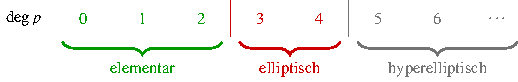
\includegraphics[width=0.9\textwidth]{papers/elliptisch/images/gradskala.pdf}
	\caption{Der Grad des Polynoms $p$ unter der Wurzel entscheidet
	über die Lösbarkeit.
	Bis Grad $2$ ist das Integral elementar, bei den Graden $3$ und
	$4$ elliptisch, ab Grad $5$ hyperelliptisch.}
	\label{fig:elliptisch:gradskala}
\end{figure}
